\documentclass[xcolor=table]{beamer}

\usetheme[secheader,compress]{Madrid} %Primary theme

\usepackage{verbatim}
\usepackage{graphicx}
\usepackage[export]{adjustbox}

%% UTM Colors
\definecolor{UTMblue}{rgb}{0.043137, 0.137254, 0.254901}
\definecolor{UTMorange}{rgb}{1.0, 0.509803, 0}

\setbeamercolor{palette primary}{bg=UTMblue,fg=white}
\setbeamercolor{palette secondary}{bg=UTMblue,fg=white}
\setbeamercolor{palette tertiary}{bg=UTMblue,fg=white}
\setbeamercolor{palette quaternary}{bg=UTMblue,fg=white}
\setbeamercolor{structure}{fg=UTMblue} % itemize, enumerate, etc
\setbeamercolor{section in toc}{fg=UTMblue} % TOC sections
\setbeamercolor{title}{fg=UTMorange}

\setbeamercolor{subsection in head/foot}{bg=UTMorange,fg=white}

%%%%%%%%%%% BEGIN MACROS %%%%%%%%%%%%%%%%%%
% frameT: Frame with title
\newcommand{\frameT}[2]{\frame{\frametitle{#1} #2}}

% frameF: Fragile frame with title
\newcommand{\frameF}[2]{
  \begin{frame}[fragile]
    \frametitle{#1}
    #2
  \end{frame}
}

% frameTop: Frame aligned t the top
\newcommand{\frameTop}[2]{\frame[t]{\frametitle{#1} #2}}


\newcommand{\tab}{\hspace{1cm}}

\newcommand{\spaceor}{\hspace{5pt} \textbf{or} \hspace{5pt}}

%%%%%%%%%%% END MACROS %%%%%%%%%%%%%%%%%%%%



\begin{document}

\title{The Deep Journey}

\author{James Blankenship and Andrew Marshall}
\institute{UT-Martin}
\date{\today}

%%%%%%%%%%% BEGIN TITLE %%%%%%%%%%%%%%%%%%
\frame{\titlepage}

 %\section{Outline}
%%%%%%%%%%%% END TITLE  %%%%%%%%%%%%%%%%%%



\section{Introduction}

  
  \section{Background}
  \frameT{Overview}{
    
  Overview of project 
  \bigskip
  \begin{enumerate}

  \item Real time combat game in Unreal Engine
    \bigskip
    \item It will be in the first person where it will be viewed from the players eyes
    \bigskip
  \item Multiple levels in game and it will be in the fantasy genre.
  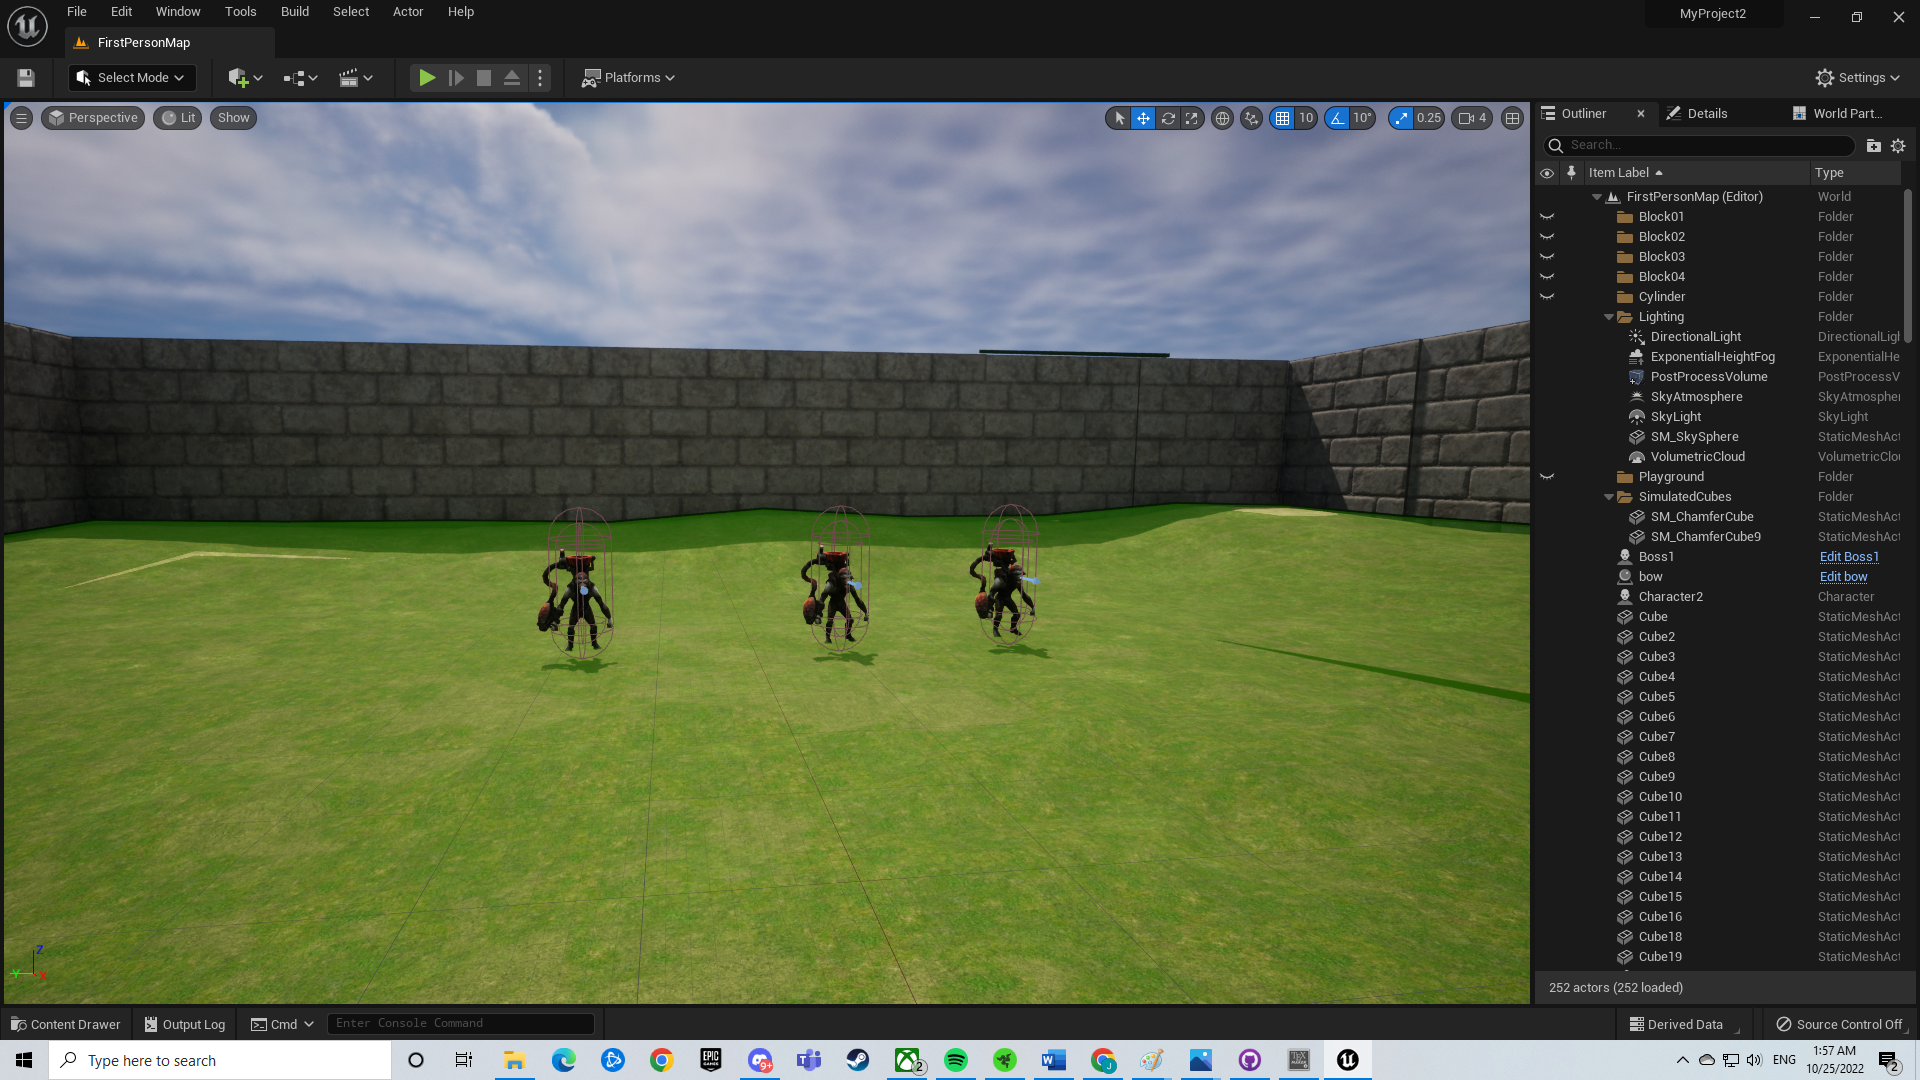
\includegraphics[width=4cm, height=4cm]{figures/Enemy.png}
   \includegraphics[width=4cm, height=4cm]{figures/Boss.png}
   
  \end{enumerate}  }
  \frameT{Overview}{
  \section{Overview cont.}
  
  Overview of Project cont.
  \begin{enumerate}
    \item Each level will focus on a enemy race.
    \bigskip
  \item Enemy types are orcs, goblins, and humans.
    \bigskip
  \item There will be weapon upgrades such as increased damage.
    \bigskip
    \item Character will have access to magic, and other abilities 
       \bigskip
    \item Magic such as pyromancy,faith magic,and sorcery.
    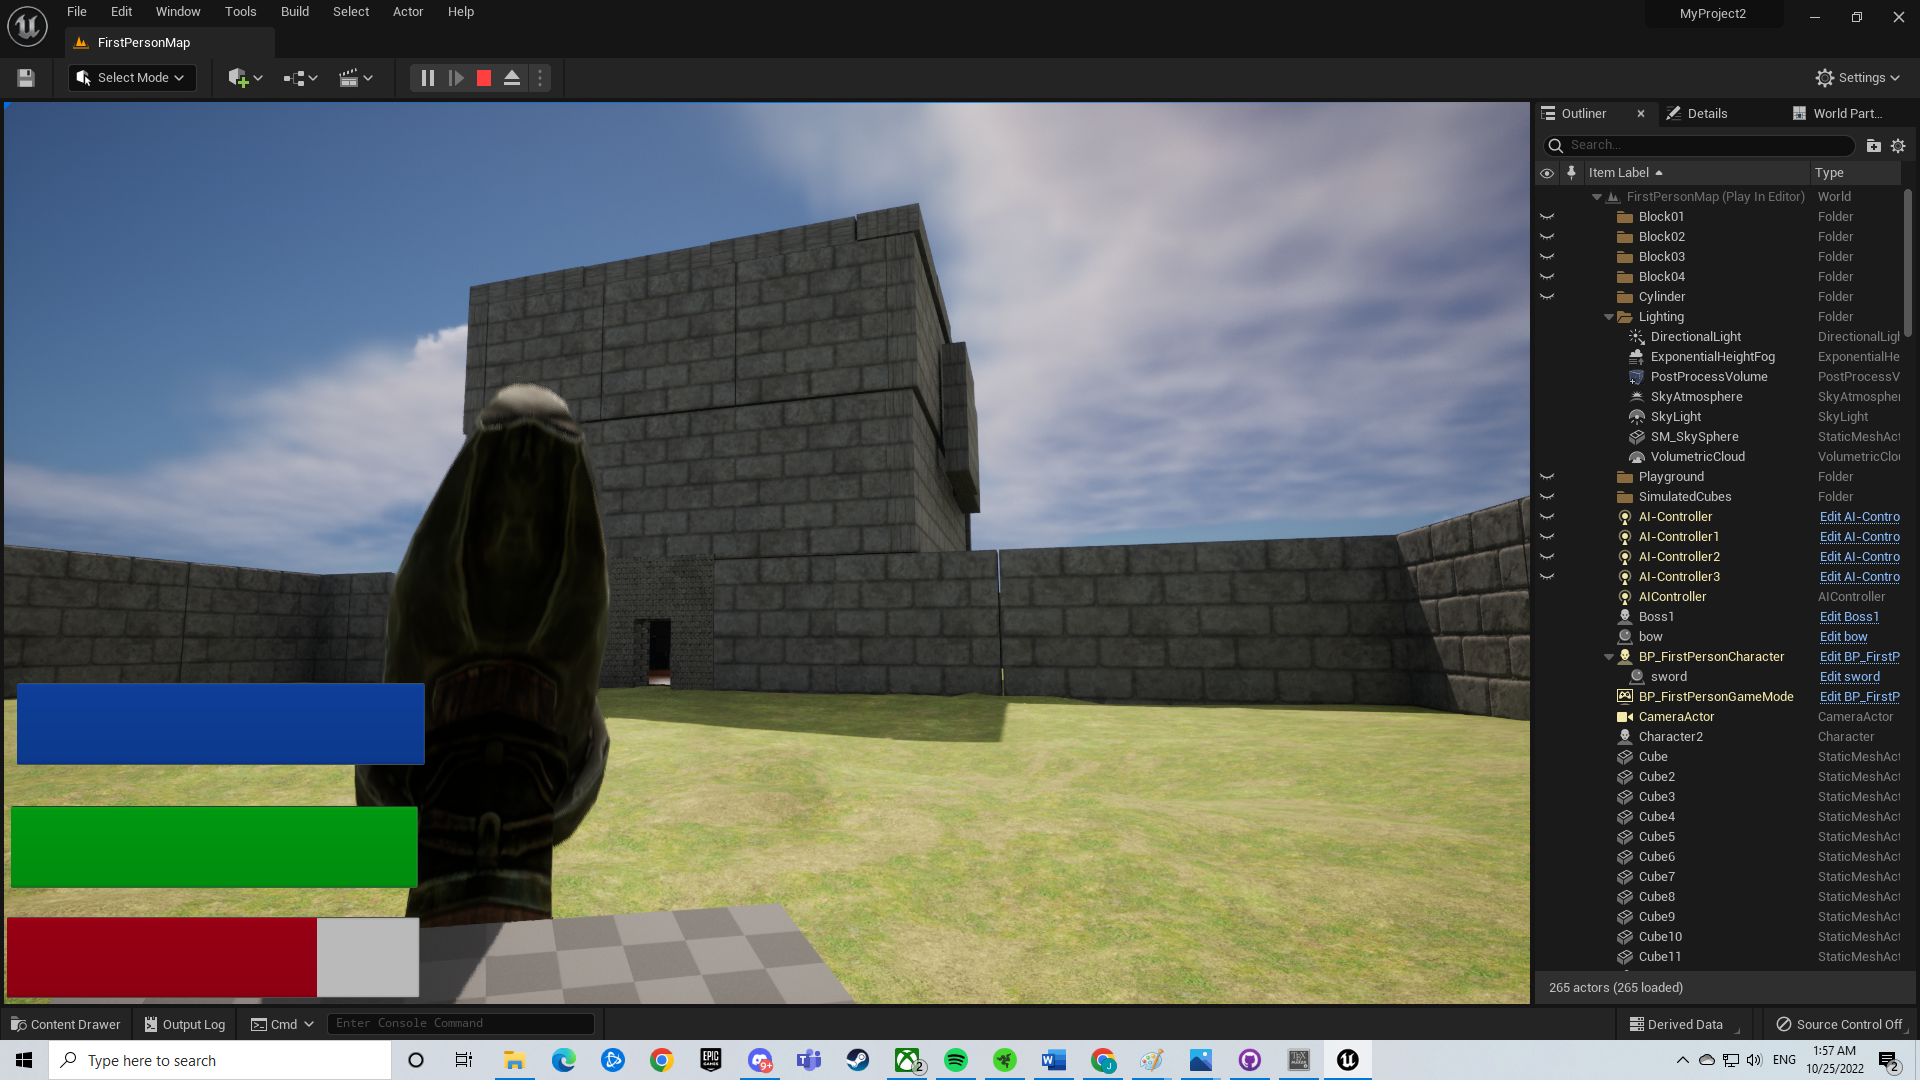
\includegraphics[width=6cm, height=4cm, center]{figures/Hammer.png}
  \end{enumerate}
  }
  


 


  \frameT{Project Goals} {
    \begin{enumerate}
  \item There are 3 different levels.
    \bigskip
  \item The three levels are  the castle level,castle basement, and the woods area.
    \bigskip
  \item The  player character will have  different classes. 
  
    \bigskip
  \item Program different AI enemies.\\
  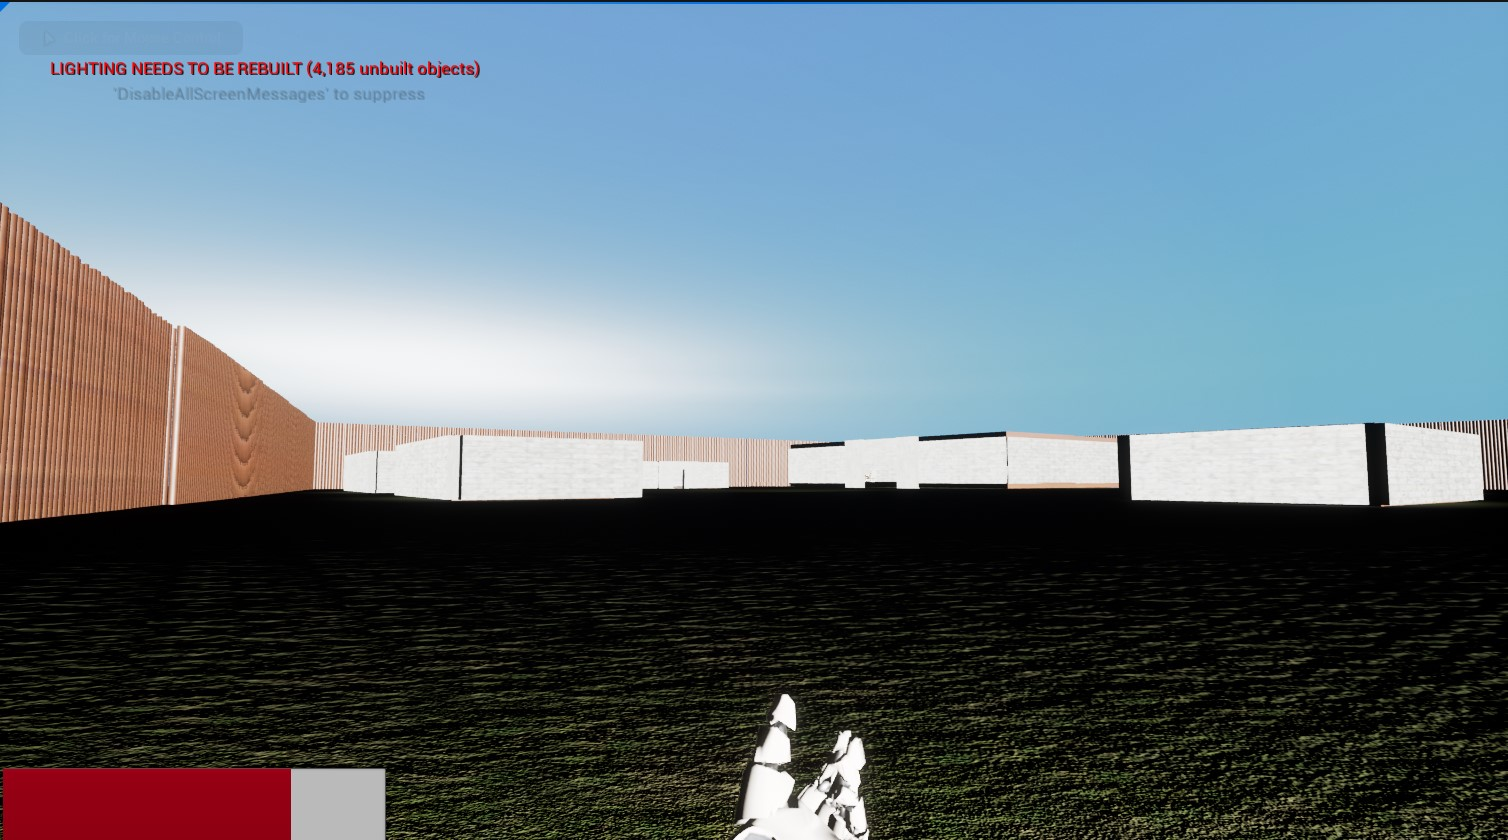
\includegraphics[width=4cm, height=4cm]{figures/woods.jpg}
  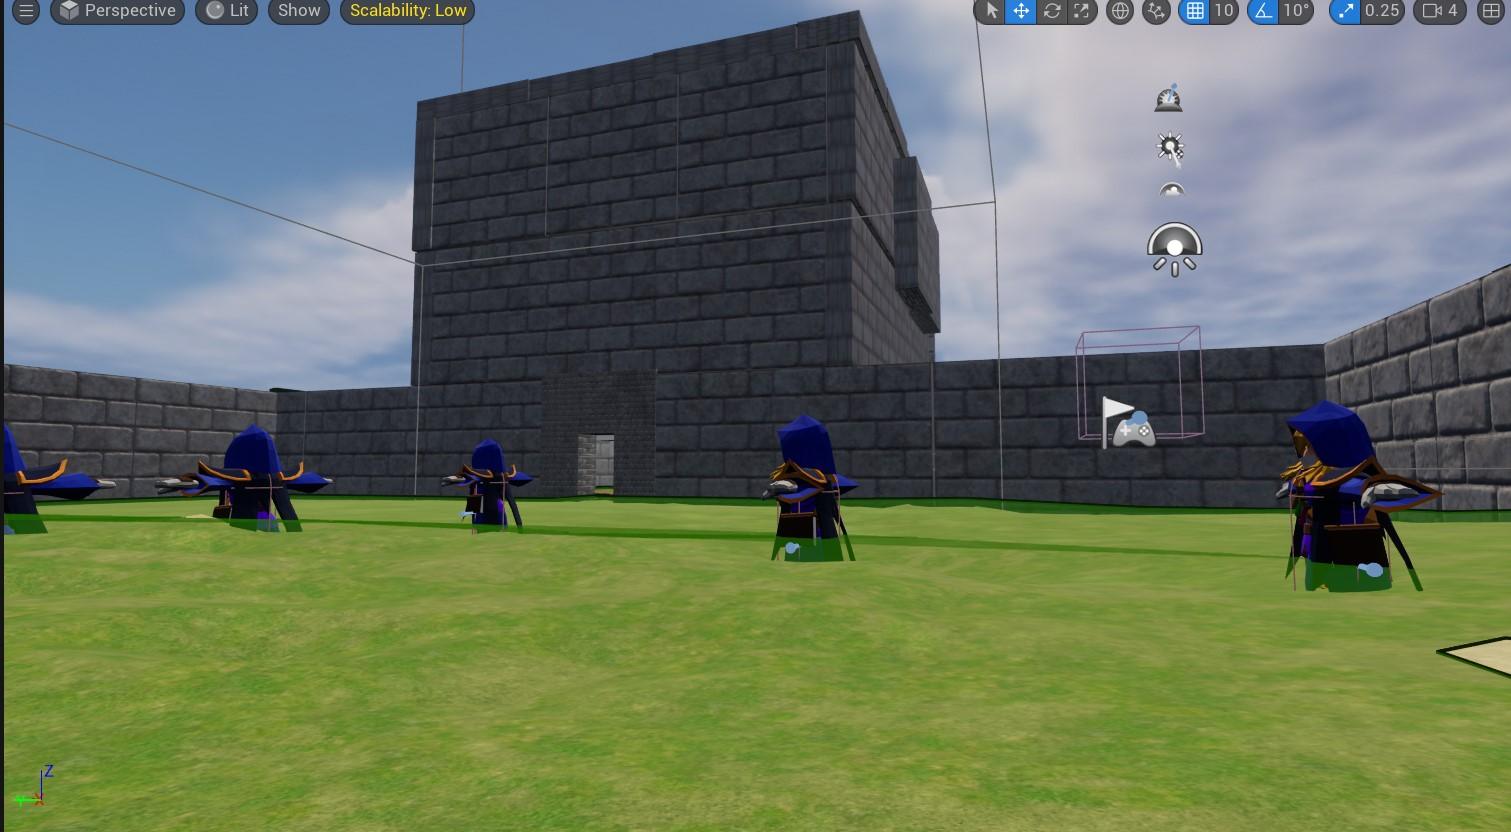
\includegraphics[width=4cm, height=4cm]{figures/castle.jpg}
  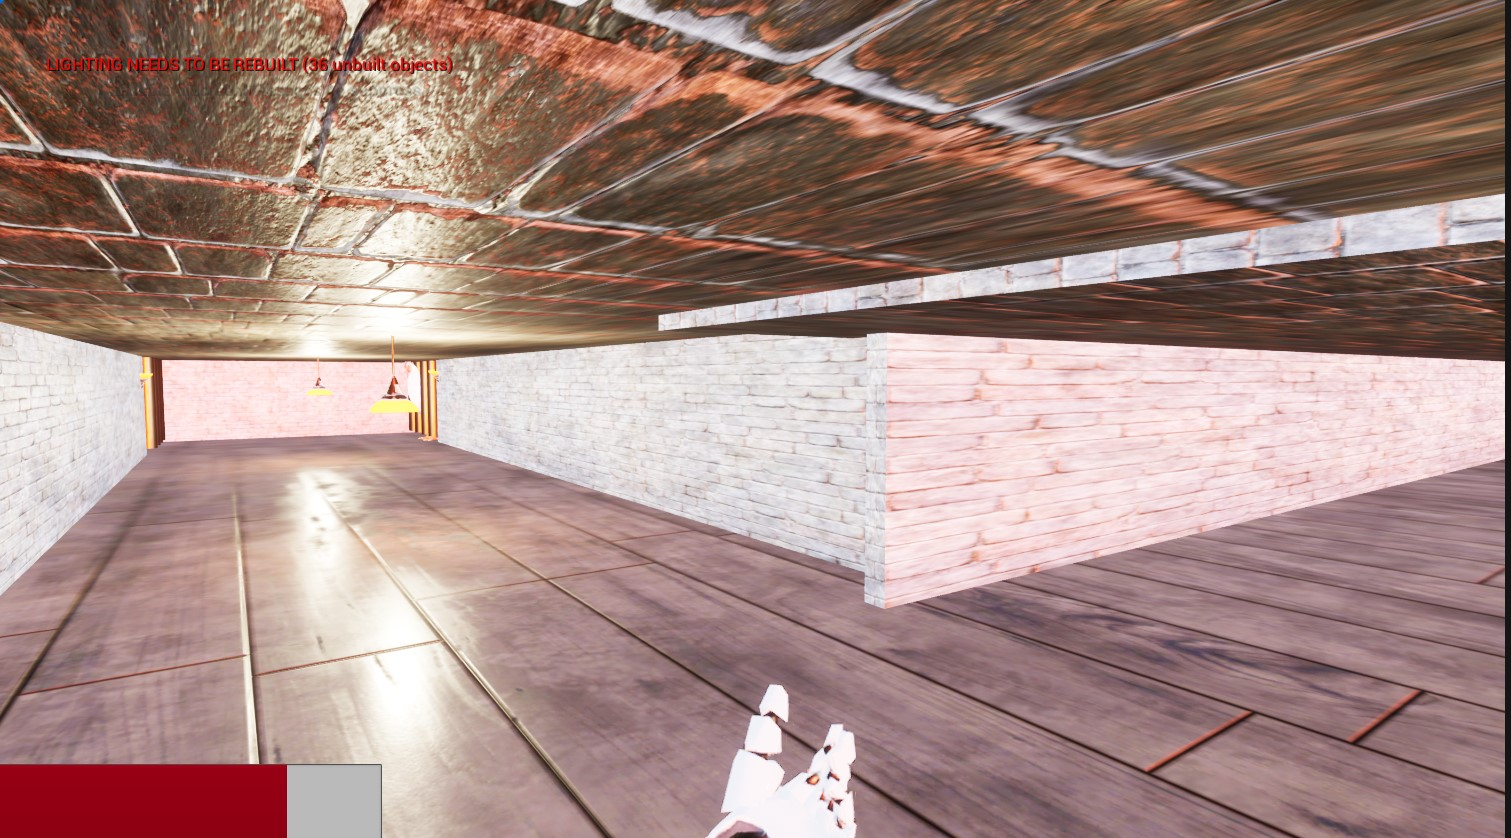
\includegraphics[width=3cm, height=4cm]{figures/basement.jpg}
    \end{enumerate}
}


 \frameT{Classes} {
    \begin{enumerate}
  \item Warrior:Melee focused with abilities to maker him a tank.
  \bigskip
  \item Mage: ranged damage dealer.
  \bigskip
  \item Melee mage: melee character with ranged abilities. 
    \end{enumerate}
}

 \frameT{Warrior} {
    \begin{enumerate}
  \item Ability 1: heals the player
  \bigskip
  \item Ability 2: gives a damage buff
  \bigskip
  \item Ultimate: Regenerates health.
    \end{enumerate}
}

 \frameT{Mage} {
    \begin{enumerate}
  \item Ability 1 :Shoots out fast moving spells that do lower damage
  \bigskip
  \item Ability 2 shoots out a close range spell that does alot of damage
  \bigskip
  \item Ultimate Regenerates resources at a faster rate.
    \end{enumerate}
}
\frameT{Castle level} {
\begin{enumerate}
  \item The starting level is the castle level.

  \bigskip

  \item The level layout will include the courtyard and the interior of the castle itself.
  
  
  \bigskip
  \item The enemies that the player will encounter are orks. \\
  \bigskip
  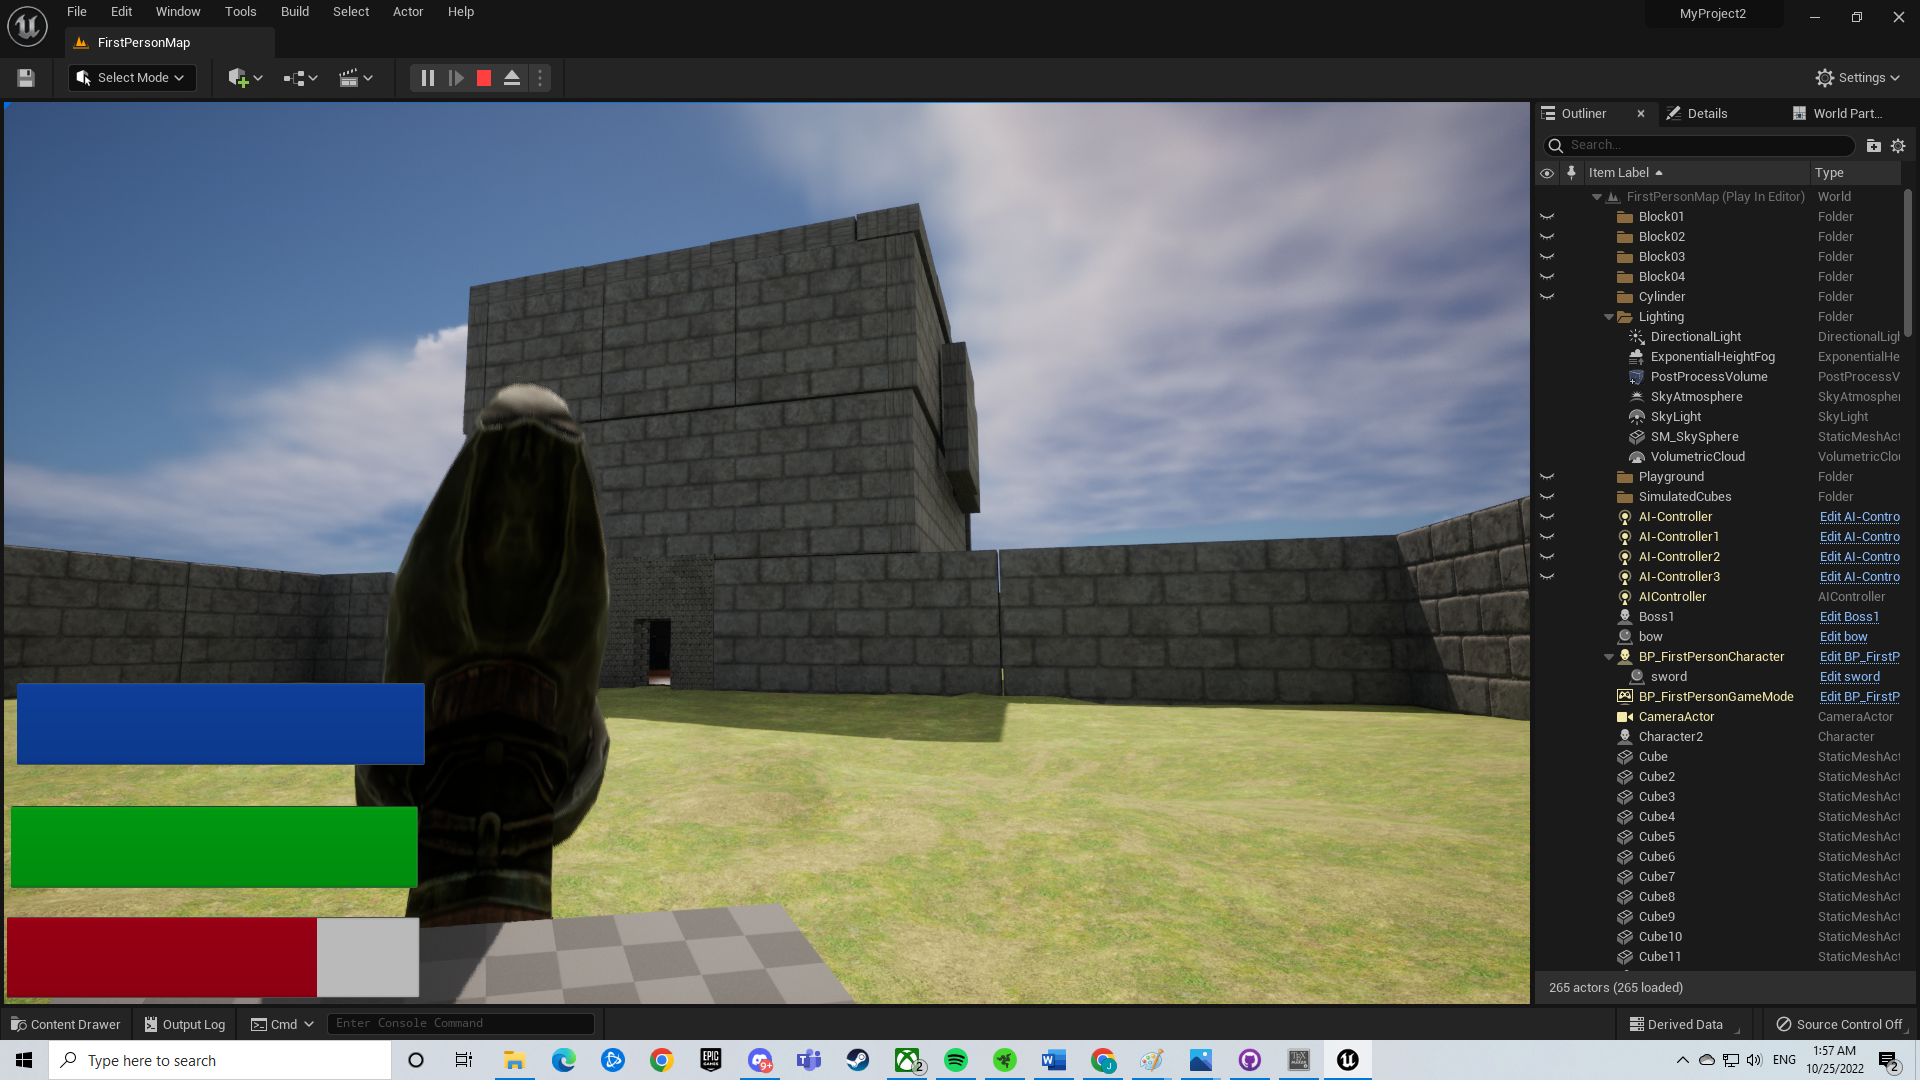
\includegraphics[width=6cm, height=4cm, center]{figures/Hammer.png}
\end{enumerate}
}
\frameT{Basement/Dungeon level} {
\begin{enumerate}
  \item The next level is the Dungeon of the castle 

  \bigskip

  \item The level lay out will include a long hallway with two corridors.
  
  \bigskip
  \item The corridors contains prison cells that have different enemies the player character will fight.\\
  \bigskip
  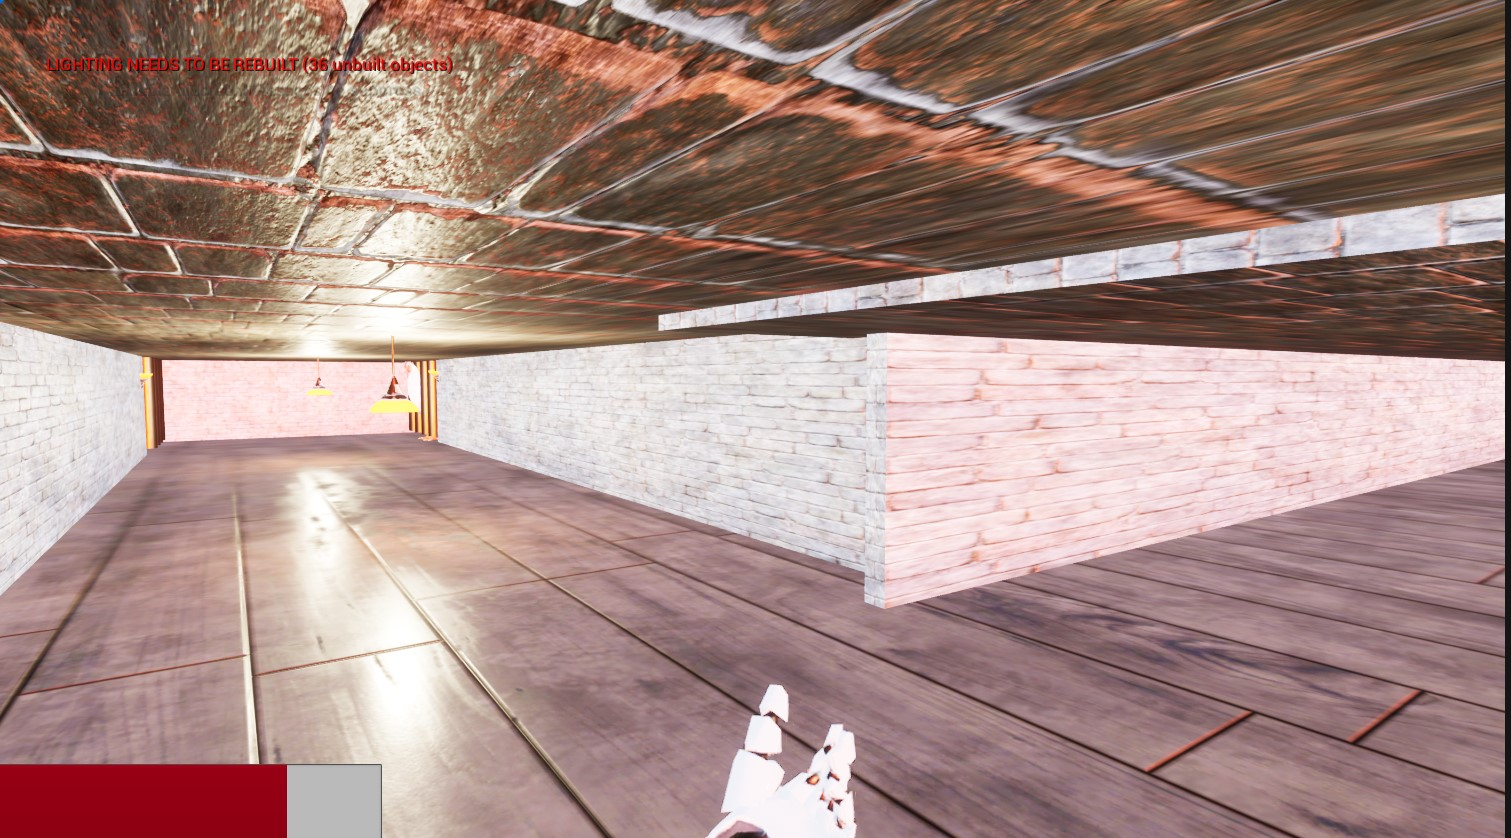
\includegraphics[width=6cm, height=4cm, center]{figures/basement.jpg}
\end{enumerate}
}
\frameT{Forest level}{
\begin{enumerate}
\item The last level is the forest area.
\bigskip
\item The level layout is a main camp area surrounded by walls.
\bigskip
\item The enemies that can be found in this level will be orks.\\
\bigskip 
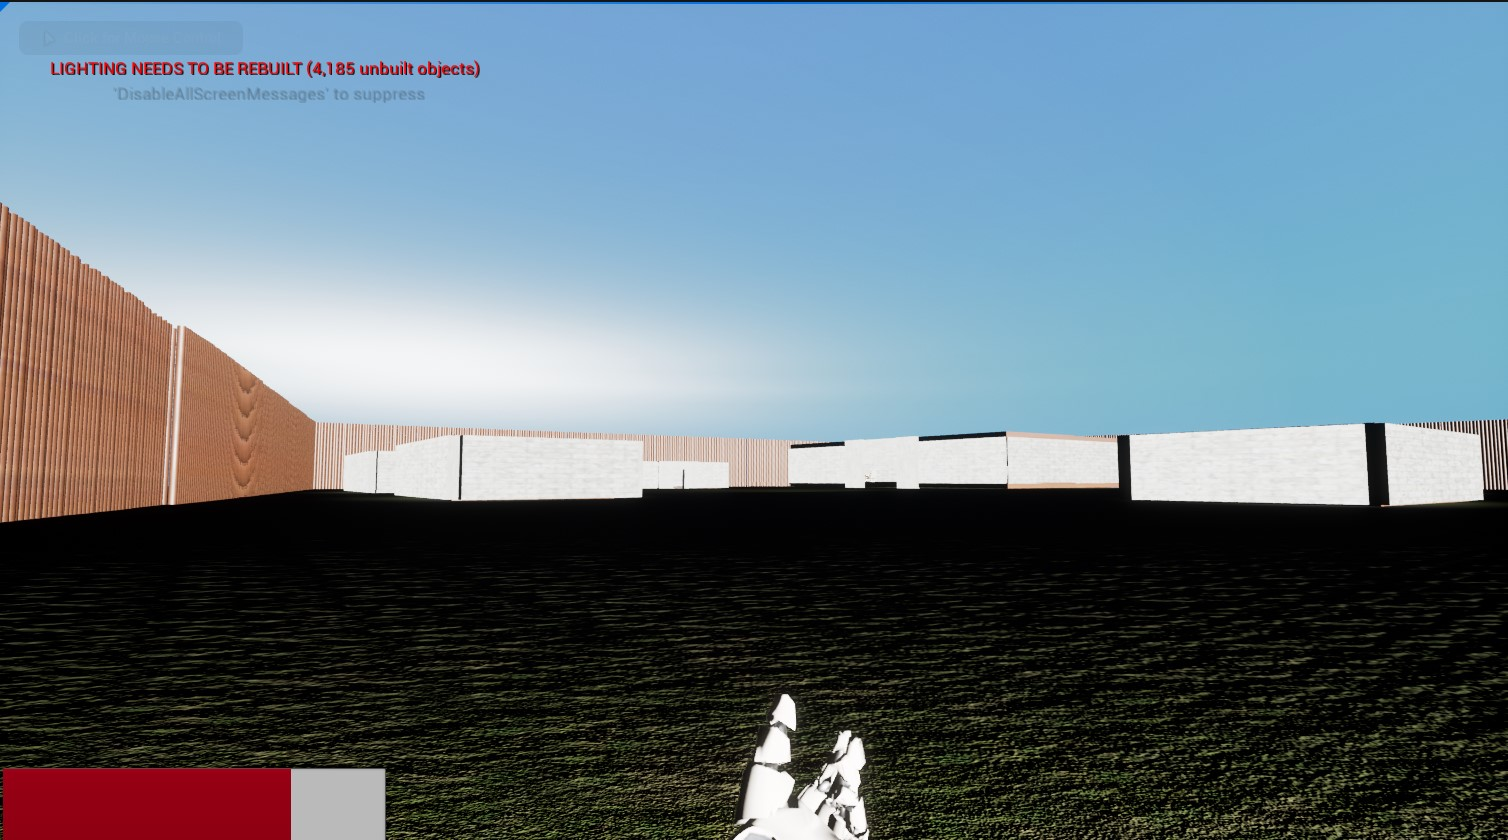
\includegraphics[width=6cm, height=4cm, center]{figures/woods.jpg}
\end{enumerate}
}

\begin{frame}[fragile]
\frametitle{Technology used}

\begin{enumerate}
    \item The game was developed using unreal engine 5.
    \bigskip
    
    \item Within the unreal engine we used trigger boxes to transition between the different levels.
    \bigskip
    \item For the enemies and different weapons we used assets from the unreal marketplace
    \bigskip
   
  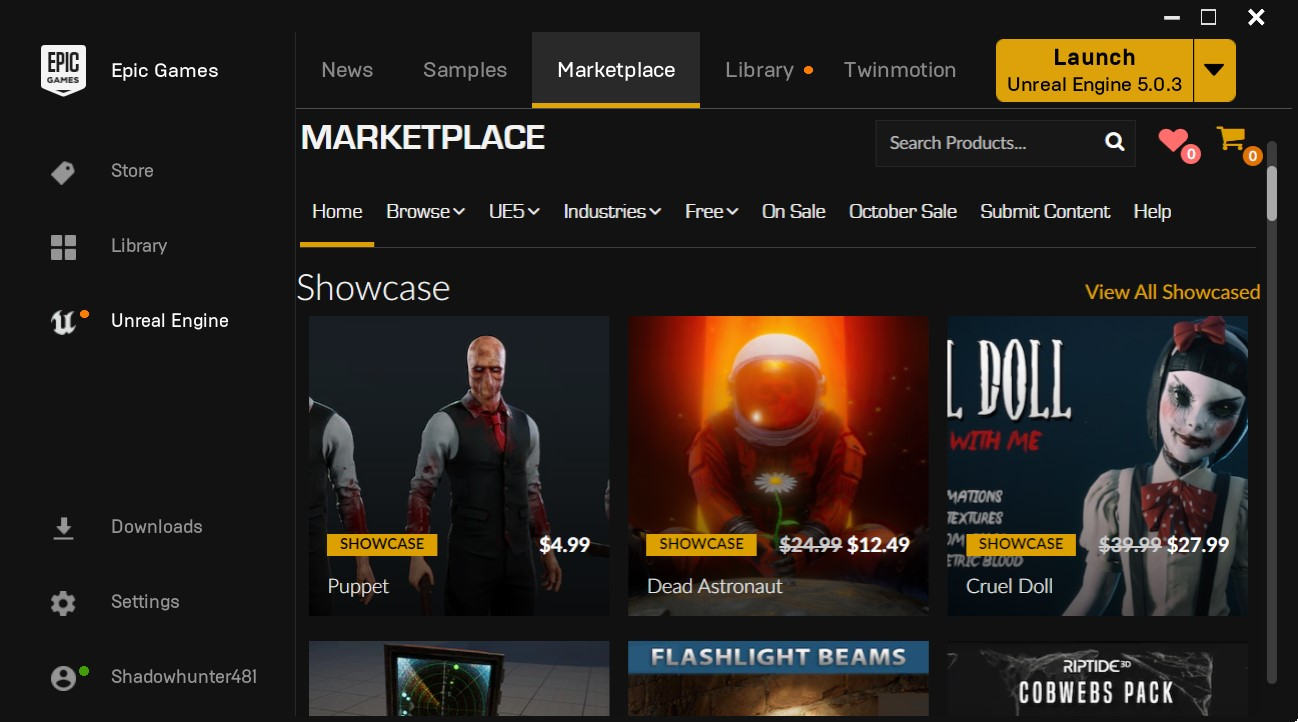
\includegraphics[width=6cm, height=4cm, center]{figures/marketplace.jpg}
  
  

    
    
  \end{enumerate}
\end{frame}
\begin{frame}[fragile]
\frametitle{Technology cont}
\begin{enumerate}
 \item For the AI and overall level we used unreals blueprint system.
    \bigskip
  \item To help with collaboration and version control we used github.
  \bigskip
    
  \item This presentation was made using latex. \\
  \bigskip
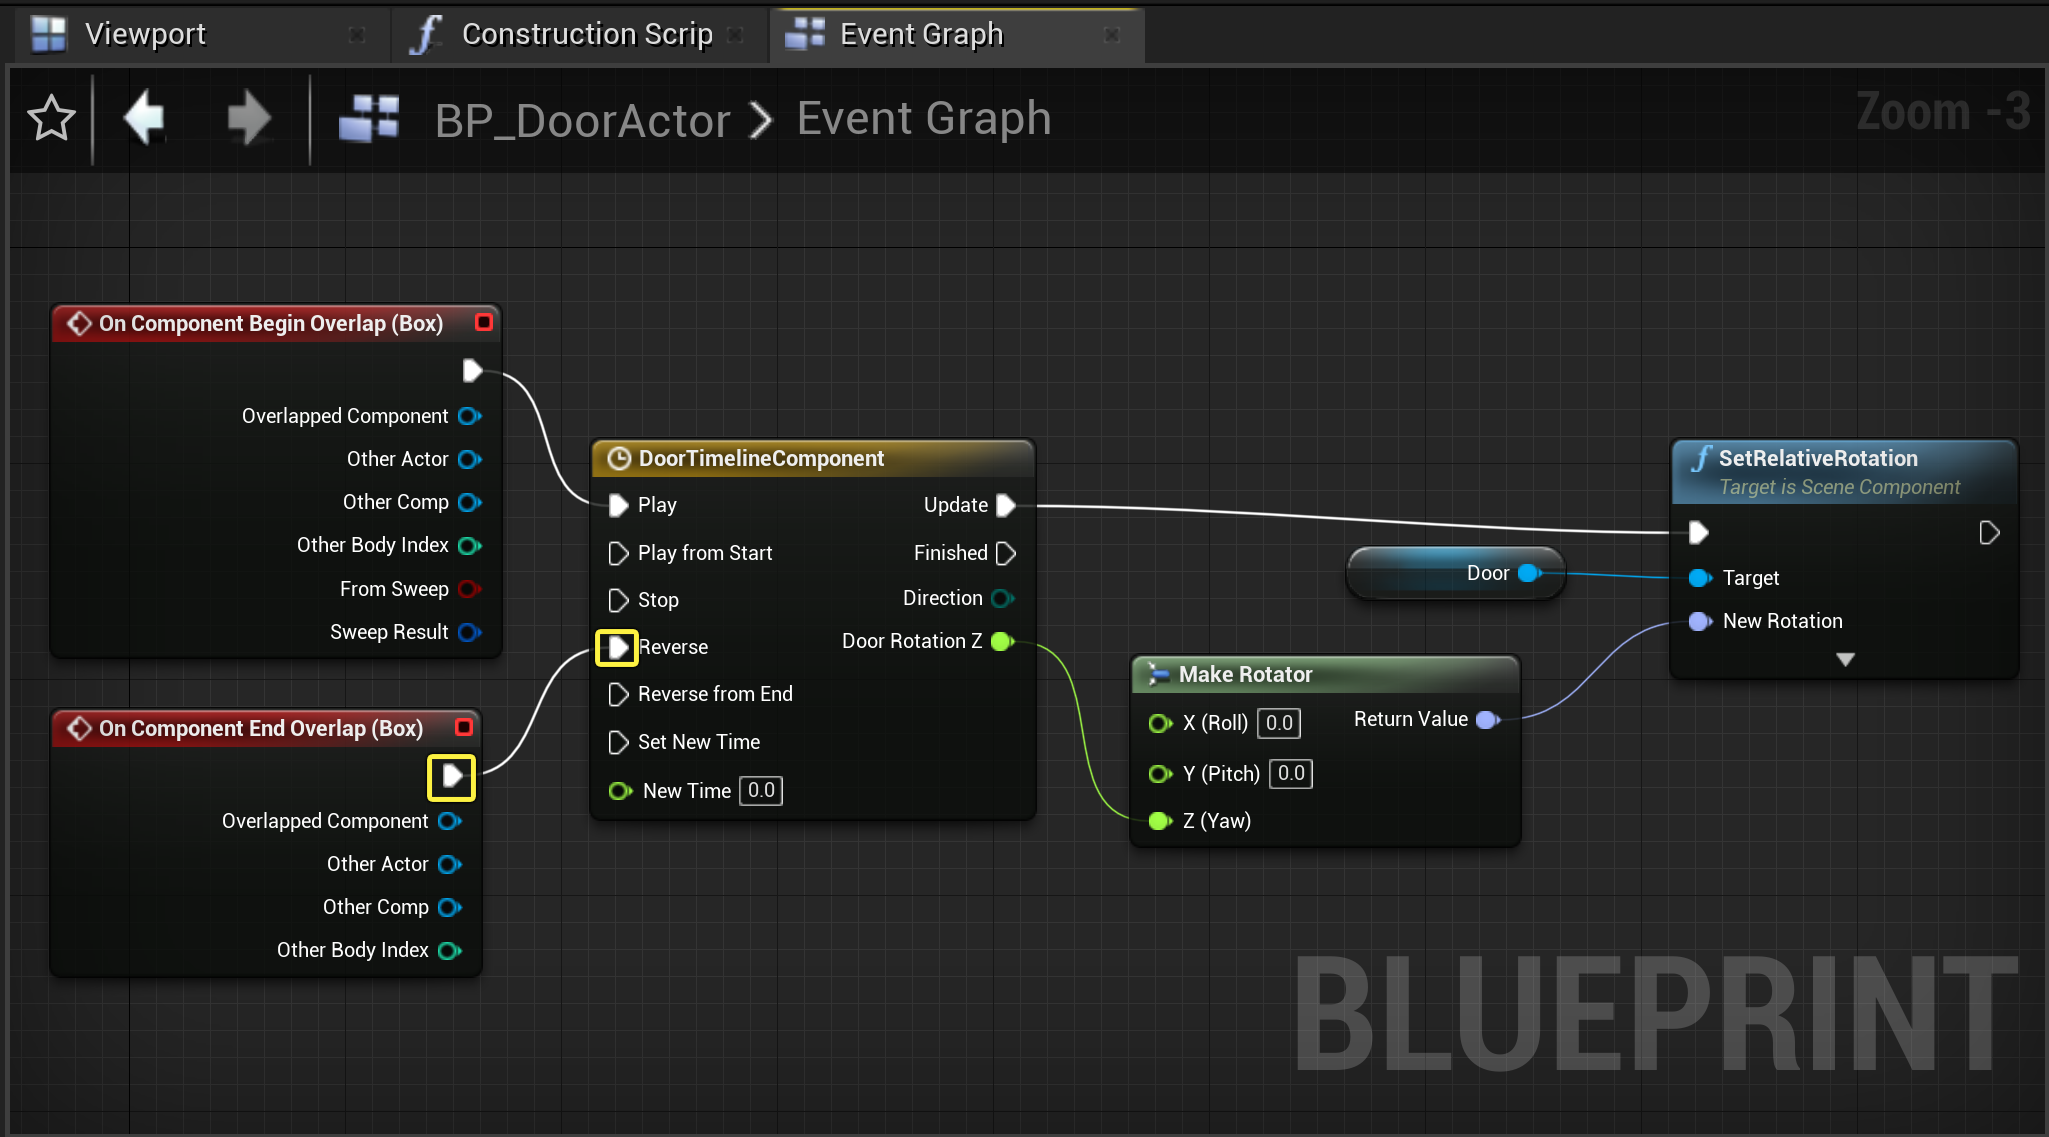
\includegraphics[width=6cm, height=4cm, center]{figures/image_21.png}
\end{enumerate}
\end{frame}


\frameT{Demo slide} {
  \begin{center}
    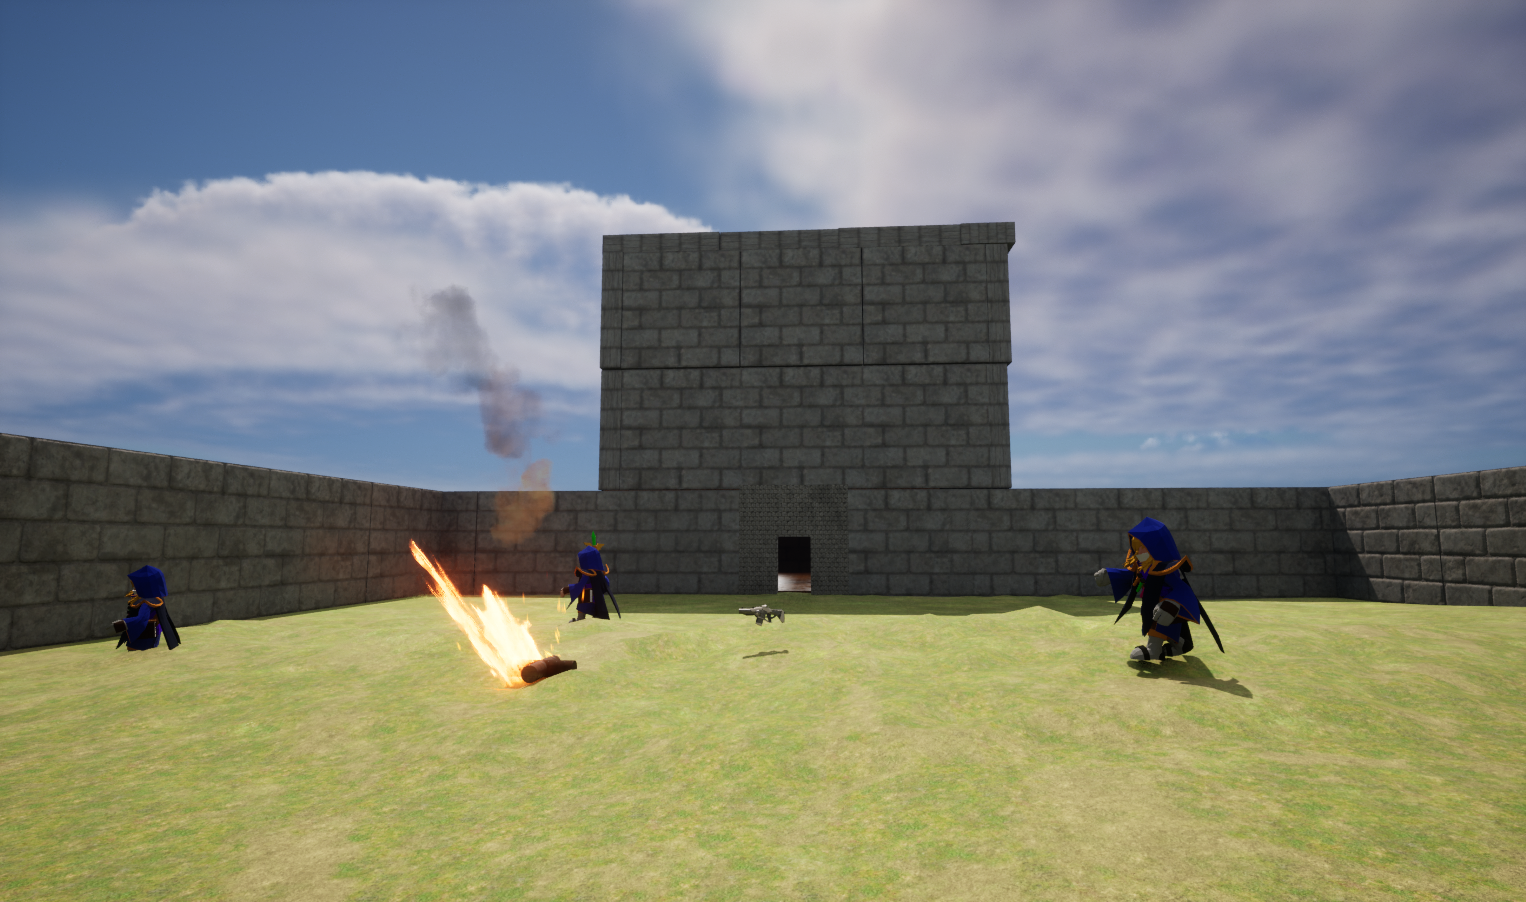
\includegraphics[width=10cm]{figures/unknown.png}
  \end{center}
}


\section{Sections--a useful organizational tool.}













\frameT{What We Learned} {
\begin{enumerate}
  \item Overall we learned unreal engine 5 and game development.

  \bigskip

  \item We learned how to do custom animation work for the enemies.
  
  \bigskip

 \item We learned how to implement AI for the enemies.
  \bigskip
 \item We also implemented a interface for the player character.
 \bigskip
 \item We figured out how to use different projectiles and weapons.
 \bigskip
 \end{enumerate}
}




\frameT{Project Development} {
   \begin{enumerate}
    \item The project started out with just the basic first-person layout. 
    \bigskip
    \item We then added the castle level. 
    \bigskip
    \item Then, we added assets from the marketplace. 
    \bigskip
    \item We added wizard that did nothing at first, and got to randomly moves.
    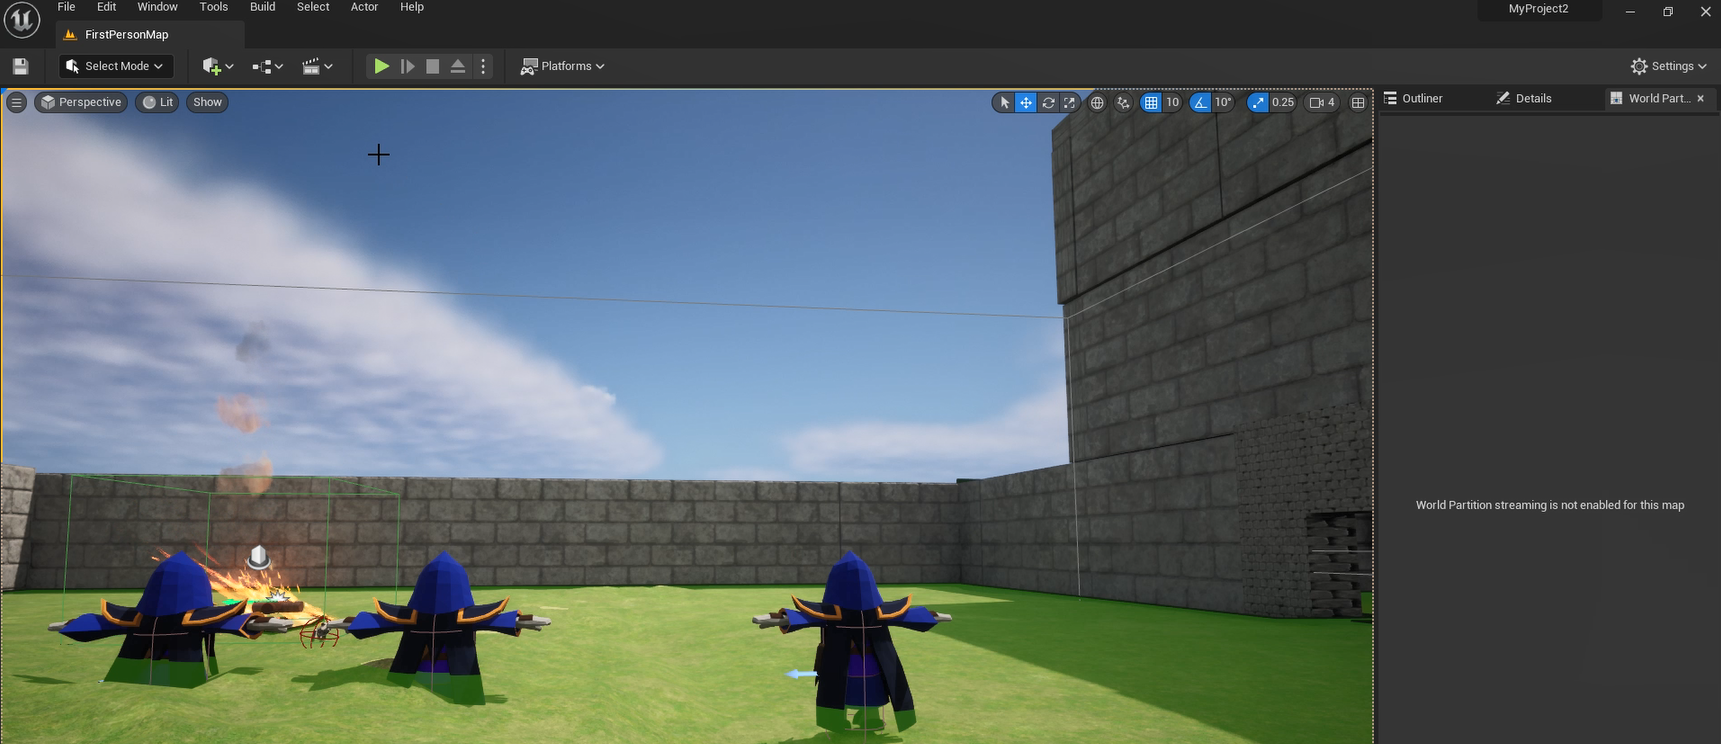
\includegraphics[width=6cm, height=4cm, center]{figures/dev1.png}
    \end{enumerate}
}

\frameT{Project Development} {
   \begin{enumerate}
    \item We figured out how to add more levels and added a basement and a woods area. 
    \bigskip
    \item We added more details to the basement area. 
    \bigskip
    \item Then, we added assets from the marketplace. 
    \bigskip
    \item We added weapons, and abilities for the classes
    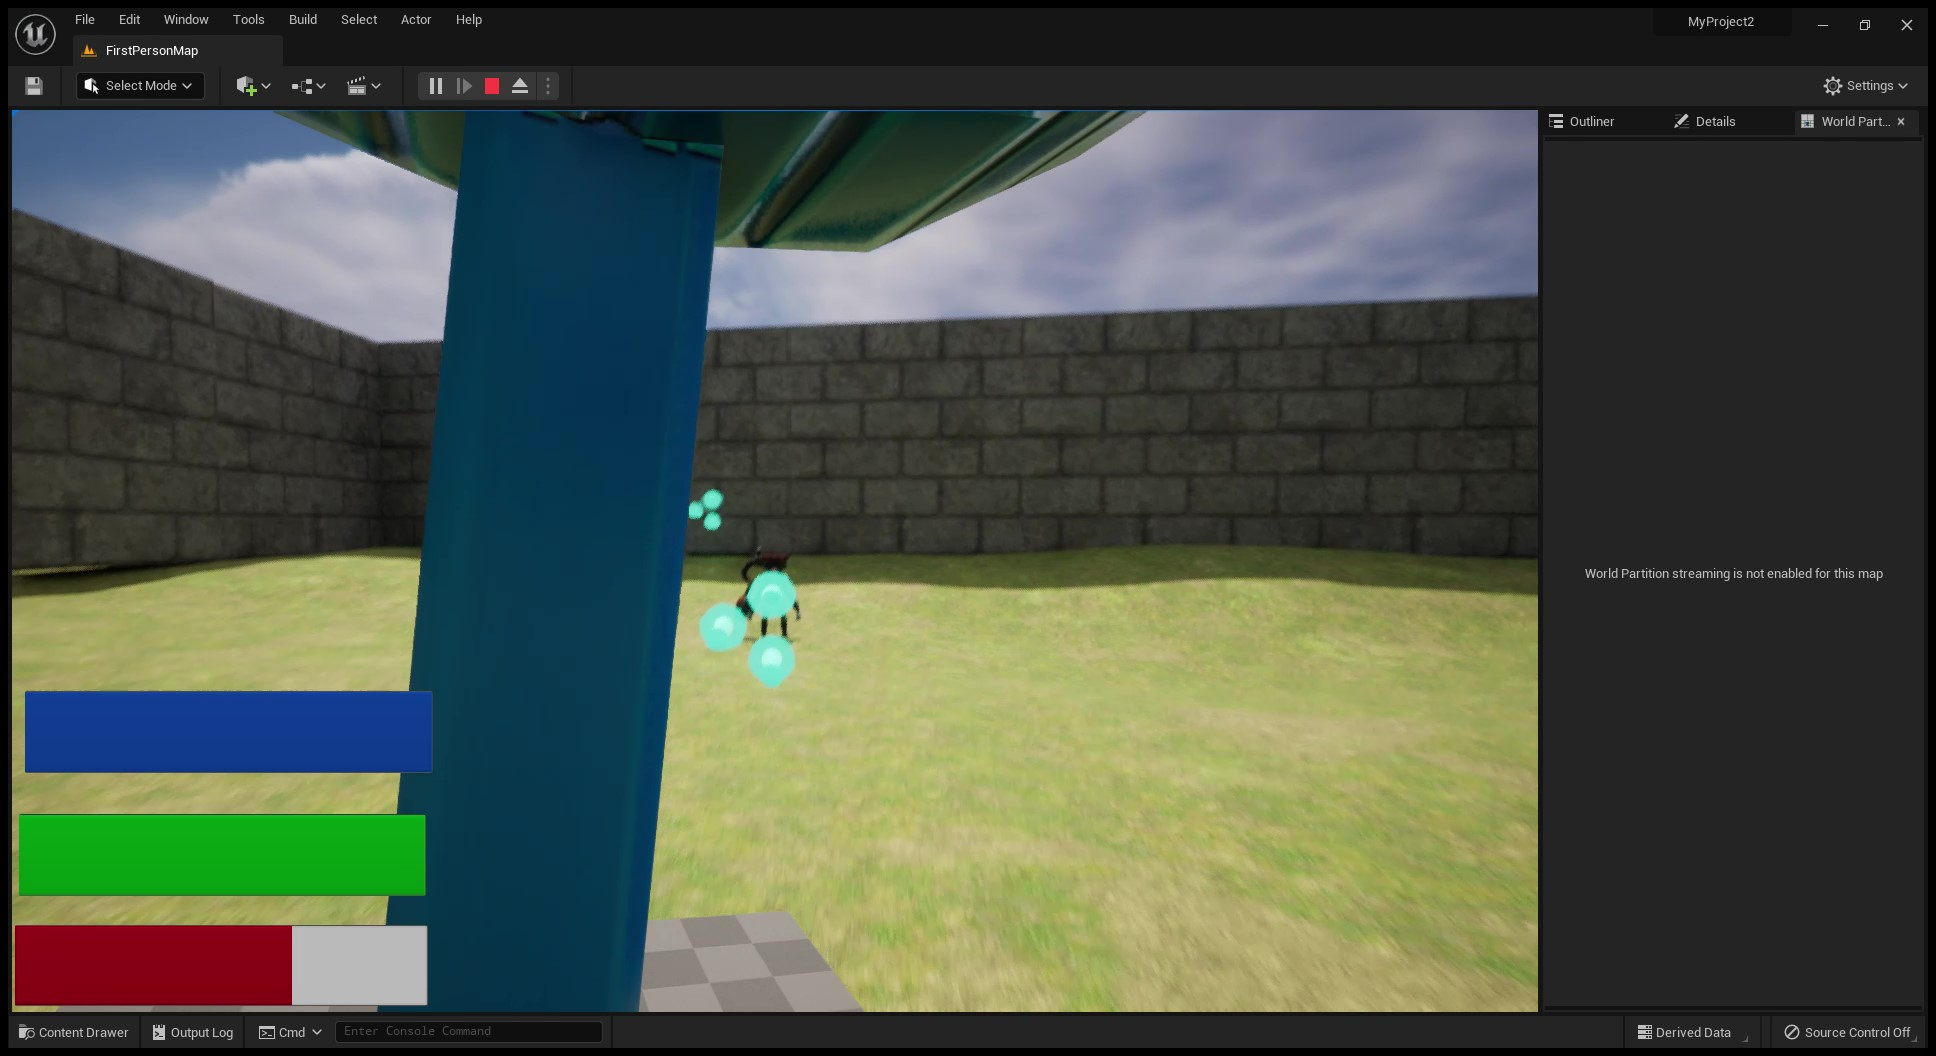
\includegraphics[width=6cm, height=4cm, center]{figures/dev2.jpg}
    \end{enumerate}
}
\frameT{Future Work} {
\begin{enumerate}
  \item Port to mobile 

  \bigskip

  \item Add more levels
  
  \bigskip

 \item Add more enemies and weapons.
 \end{enumerate}
}
\frameT{Summary}{
  \begin{enumerate}
    \item Any Questions or comments?
    \bigskip
    \item Below is our contact info
    \bigskip
    \item jesamars@ut.utm.edu or jamcblan@ut.utm.edu
    \bigskip
    \item https://github.com/James-Blankenship4276/CSCI-Senior-Project
    
\includegraphics[width=5cm, height=4cm, center]{figures/qrcode_github.com.png}
    \end{enumerate}
}



%\frameF{fragile test} {
%}

%% \frameF{Prolog Family Tree} {
%% \begin{verbatim}
%% hello
%% \end{verbatim}



%% }

%Empty Page
%\frameT{Frame 1}{
%}  


\end{document}
